\documentclass[]{fim-uhk-thesis}
%\documentclass[english]{fim-uhk-thesis} % without assignment - for the work start to avoid compilation problem
% * Je-li práce psaná v anglickém jazyce, je zapotřebí u třídy použít
%   parametr english následovně:
%   If thesis is written in English, it is necessary to use
%   parameter english as follows:
%      \documentclass[english]{fim-uhk-thesis}
% * Je-li práce psaná ve slovenském jazyce, je zapotřebí u třídy použít
%   parametr slovak následovně:
%   If the work is written in the Slovak language, it is necessary
%   to use parameter slovak as follows:
%      \documentclass[slovak]{fim-uhk-thesis}
% * Je-li práce psaná v anglickém jazyce se slovenským abstraktem apod.,
%   je zapotřebí u třídy použít parametry english a enslovak následovně:
%   If the work is written in English with the Slovak abstract, etc.,
%   it is necessary to use parameters english and enslovak as follows:
%      \documentclass[english,enslovak]{fim-uhk-thesis}

% Základní balíčky jsou dole v souboru šablony fim-uhk-thesis.cls
% Basic packages are at the bottom of template file fim-uhk-thesis.cls
% zde můžeme vložit vlastní balíčky / you can place own packages here



%---rm---------------
\renewcommand{\rmdefault}{lmr}%zavede Latin Modern Roman jako rm / set Latin Modern Roman as rm
%---sf---------------
\renewcommand{\sfdefault}{qhv}%zavede TeX Gyre Heros jako sf
%---tt------------
\renewcommand{\ttdefault}{lmtt}% zavede Latin Modern tt jako tt

% vypne funkci šablony, která automaticky nahrazuje uvozovky,
% aby nebyly prováděny nevhodné náhrady v popisech API apod.
% disables function of the template which replaces quotation marks
% to avoid unnecessary replacements in the API descriptions etc.
\csdoublequotesoff



\usepackage{url}

\def\UrlBreaks{\do\/\do-}
\usepackage{breakurl}


% =======================================================================
% balíček "hyperref" vytváří klikací odkazy v pdf, pokud tedy použijeme pdflatex
% problém je, že balíček hyperref musí být uveden jako poslední, takže nemůže
% být v šabloně
% "hyperref" package create clickable links in pdf if you are using pdflatex.
% Problem is that this package have to be introduced as the last one so it
% can not be placed in the template file.

  \usepackage{color}
  \usepackage[unicode,colorlinks,hyperindex,plainpages=false,urlcolor=black,linkcolor=black,citecolor=black]{hyperref}
  \definecolor{links}{rgb}{0,0,0}
  \definecolor{anchors}{rgb}{0,0,0}
  \def\AnchorColor{anchors}
  \def\LinkColor{links}
  \def\pdfBorderAttrs{/Border [0 0 0] } % bez okrajů kolem odkazů / without margins around links
  \pdfcompresslevel=9

% Řešení problému, kdy klikací odkazy na obrázky vedou za obrázek
% This solves the problems with links which leads after the picture
\usepackage[all]{hypcap}

\projectinfo{
  %Prace / Thesis
  % TODO WRITER: choose thesis type
  project={BP},            %typ práce BP/SP/DP/DR  / thesis type (SP = term project)
  % TODO WRITER: enter year of submission
  year={2022},             % rok odevzdání / year of submission
  date=\today,             % datum odevzdání / submission date
  %Nazev prace / thesis title
  % TODO WRITER: enter czech title
  title.cs={Český název},  % název práce v češtině či slovenštině (dle zadání) / thesis title in czech language (according to assignment)
  % TODO WRITER: enter english title
  title.en={English title}, % název práce v angličtině / thesis title in english
  %Autor / Author
  % TODO WRITER: enter author
  author.name={Pepa},   % jméno autora / author name
  author.surname={Novák},   % příjmení autora / author surname
  % TODO WRITER: enter field
  author.field={Aplikovaná Informatika},   % obor
  %Ustav / Department
  % TODO WRITER: enter deparment
  department={KIT}, % doplňte příslušnou zkratku dle ústavu na zadání: DEF / fill in appropriate abbreviation of the department according to assignment: DEF
  % Školitel / supervisor
  % TODO WRITER: enter supervisor
  supervisor.name={Adam},   % jméno školitele / supervisor name
  supervisor.surname={Slabý},   % příjmení školitele / supervisor surname
  supervisor.title.p={Ing.},   %titul před jménem (nepovinné) / title before the name (optional)
  supervisor.title.a={CSc.},
  % Anotace
  % TODO WRITER: enter czech annotation
  annotation.cs={
    Lorem ipsum dolor sit amet, consectetur adipiscing elit. Phasellus sit amet ornare diam,
    id consequat diam. Integer accumsan eu mauris eu rutrum. Donec scelerisque eu nibh non
    aliquam. Sed at nunc vel magna dignissim laoreet sit amet id sapien. Donec pharetra,
    diam et molestie fringilla, magna eros luctus metus, a dapibus erat nulla ullamcorper
    lectus. In augue tellus, sagittis condimentum odio quis, consectetur vestibulum nisl.
    Nam euismod hendrerit efficitur. Cras eu ipsum at neque pretium porttitor. Mauris
    fermentum dolor a libero feugiat hendrerit. Mauris venenatis orci molestie vulputate
    semper. Duis finibus accumsan ultricies. Pellentesque viverra tortor posuere venenatis
    eleifend. Etiam dignissim mattis iaculis.
  },
  % TODO WRITER: enter english annotation
  annotation.en={
    Lorem ipsum dolor sit amet, consectetur adipiscing elit. Phasellus sit amet ornare diam,
    id consequat diam. Integer accumsan eu mauris eu rutrum. Donec scelerisque eu nibh non
    aliquam. Sed at nunc vel magna dignissim laoreet sit amet id sapien. Donec pharetra,
    diam et molestie fringilla, magna eros luctus metus, a dapibus erat nulla ullamcorper
    lectus. In augue tellus, sagittis condimentum odio quis, consectetur vestibulum nisl.
    Nam euismod hendrerit efficitur. Cras eu ipsum at neque pretium porttitor. Mauris
    fermentum dolor a libero feugiat hendrerit. Mauris venenatis orci molestie vulputate
    semper. Duis finibus accumsan ultricies. Pellentesque viverra tortor posuere venenatis
    eleifend. Etiam dignissim mattis iaculis.
  },
  % TODO WRITER: enter declaration if you want something else
  declaration={
    Prohlašuji, že jsem bakalářskou práci zpracoval samostatně a s použitím uvedené literatury.
  },
  % TODO WRITER: enter acknowledgment, you can only change name of the supervisor
  acknowledgment={
    Tímto bych chtěl poděkovat vedoucímu mé práce Ing. Adamu Slabému CSc. za odborné vedení
    práce, poskytnuté rady a přínosné konzultace, také mým přátelům za jejich pomoc a podporu.
  },
%(external submitter, consultant, etc.).},
  faculty={FIM},
  department={KIT}
}

% řeší první/poslední řádek odstavce na předchozí/následující stránce
% solves first/last row of the paragraph on the previous/next page
\clubpenalty=10000
\widowpenalty=10000

% @SEE http://ftp.cvut.cz/tex-archive/macros/latex/contrib/acro/acro-manual.pdf
% TODO WRITER: acronyms

\DeclareAcronym{DNN}{
  short=DNN,
  long=deep neuron network
}

\DeclareAcronym{URL}{
  short=URL,
  long=Uniform Resource Locator
}


% začátek dokumentu
\begin{document}
  % Vysazeni titulnich stran / Typesetting of the title pages
  % ----------------------------------------------
  \maketitle
  % Obsah
  % ----------------------------------------------
  \setlength{\parskip}{0pt}

  \thispagestyle{empty}
  {\hypersetup{hidelinks}\tableofcontents}

  % vynechani stranky v oboustrannem rezimu
  % Skip the page in the two-sided mode
  \iftwoside
    \cleardoublepage
  \fi

  % Text prace / Thesis text
  % ----------------------------------------------
  \setcounter{page}{0}
  \section{Úvod}

% TODO WRITER: text

Zde vysvětlit problémovou situaci a otázky, které se budou v bakalářské/diplomové práci řešit.

\section{Cíl práce}

% TODO WRITER: text

Smysl a účel, výzkumné otázky.

\section{Metodika zpracování}

% TODO WRITER: text

Cíle, hypotézy/ výzkumné otázky, způsob hledání odpovědí na výzkumné otázky včetně metodiky vlastního výzkumu/šetření, literární rešerše.

\section{Vlastní text práce}

% TODO WRITER: text

Vlastní řešení dokládá student zpravidla v několika kapitolách. Podle charakteru práce musí student uvážit, zda informace
netextové povahy (data, tabulky, obrázky atd.) bude uvádět přímo v textu, nebo je zařadí až za celou práci ve formě příloh, či bude kombinovat oba způsoby.
Více podrobností viz Metodické pokyny pro vypracování bakalářských a diplomových prací (zveřejňované formou výnosů děkana)
a v kurzu MES – Metodologický seminář.

	\subsection{Podkapitola}

	Text podkapitoly.

	Následuje ukázka nějakého seznamu:
	\begin{itemize}
		\item fotografie/avatar,
		\item kategorizační štítky,
		\item popisek.
	\end{itemize}

		\subsubsection{Podpodkapitola}

		Lorem ipsum dolor sit amet, consectetur adipiscing elit. Phasellus sit amet ornare diam, id consequat diam.

			\nlparagraph{Paragraf}

			\noindent Ukázka prvního odstavce v paragrafu. Lorem ipsum dolor sit amet, consectetur adipiscing elit. Phasellus sit amet ornare diam, id consequat diam.

			Následuje použití citací: Citace \cite{html_hypertext_markup_language}, \cite{hibernate_docs}, \cite{ddd_quickly}.
			Použití zkratek se rozděluje na první použítí a další použití: první použití \firstac{URL} a další použítí \ac{URL}.

			Použití obrázku je jednoduché, zadáme název souboru, šířku, popisek a zdroj:

			\cntcapfigure{rovnovaha_paka}{8cm}{Páka rovnováhy vzhledu.}{\cite{vizualni_rovnovaha}}

			V případně, že autor je i autor obrázku:

			\cntcapfigure{uhk}{\linewidth}{Toto je UHK.}{[autor]}

			Blok kódu může vypadat takto:

			\begin{codeblock}
				\begin{verbatim}
@Mapper
public interface AccountDao {
  @Select({
    "select *",
    "from " + Account.TABLE_NAME,
    "where email = #{email}"
  })
  Optional<Account> findByEmail(String email);
}
				\end{verbatim}
				\captionsource{Ukázka bloku kódu.}{[autor]}
			\end{codeblock}

			Tabulka zas může vypadat takto:

			\begin{table}[hbt!]
				\captionsource{Ukázková tabulka.}{[autor]}
				\centering
				\begin{tabular}{| l | r | r | r | }
					\hline
					&        psnr &      ssim &      doba  \\
					model &       (db)    &           & gen. (s) \\
					\hline
					bik. int. & 28.3155 & 0.8566 & 0.0322 \\
					nn1000    & 30.1461 & 0.9043 & 0.8109 \\
					nn1001    & 30.0324 & 0.9023 & 0.7486 \\
					nn1002    & \textbf{30.1886} & \textbf{0.9046} & 1.1731 \\
					nn1003    & 30.0390 & 0.9030 & 1.1320 \\
					nn1004    & 24.9772 & 0.7172 & 4.4367 \\
					nn1005    & 26.1629 & 0.8004 & 4.0475 \\
					nn1006    & 27.9129 & 0.8438 & 4.0683 \\
					nn1007    & 27.5834 & 0.8360 & 4.2082 \\
					\hline
				\end{tabular}
			\end{table}

			\newpage

			Další text

\section{Závěry a doporučení}

% TODO WRITER: text

Kritická diskuze nad výsledky, ke kterým autor dospěl (soulad výsledků  literaturou či předpoklady;
výsledky a okolnosti, které zvláště ovlivnily předkládanou práci atd.). Je vhodné naznačit i případné další
(popř. alternativní) možnosti zkoumání dané problematiky a otevřené problémy pro další studium.


  \iftwoside
    \cleardoublepage
  \fi

  % Pouzita literatura / Bibliography
  % ----------------------------------------------

\ifslovak
  \makeatletter
  \def\@openbib@code{\addcontentsline{toc}{section}{Literatúra}}
\else
  \ifczech
    \makeatletter
    \def\@openbib@code{\addcontentsline{toc}{section}{Seznam použitých zdrojů}}
  \else
    \makeatletter
    \def\@openbib@code{\addcontentsline{toc}{section}{Bibliography}}
  \fi
\fi
  \makeatother
  \begin{flushleft}
  \label{references}

  \bibliographystyle{bibstyle}
  \bibliography{literature}
  \end{flushleft}

  \newpage

  % vynechani stranky v oboustrannem rezimu
  % Skip the page in the two-sided mode
  \iftwoside
    \cleardoublepage
  \fi

  \ifslovak
   \addcontentsline{toc}{section}{Zoznam zkratek}
  \else
    \ifczech
      \addcontentsline{toc}{section}{Seznam zkratek}
    \else
      \addcontentsline{toc}{section}{List of Abbreviations}
    \fi
  \fi
  \startcontents[section]
  \label{abb}
  \setlength{\parskip}{0pt}
  % seznam příloh / list of appendices
  % \printcontents[section]{l}{0}{\setcounter{tocdepth}{2}}

  \printacronyms[name=Seznam zkratek,heading=section*]

  \newpage
  % vynechani stranky v oboustrannem rezimu
  \iftwoside
    \cleardoublepage
  \fi

  % Seznam obrazku a tabulek (pokud prace obsahuje velke mnozstvi obrazku, tak se to hodi)
  % List of figures and list of tables (if the thesis contains a lot of pictures, it is good)

  \addcontentsline{toc}{section}{Seznam obrázků}
  \ifczech
  \renewcommand\listfigurename{Seznam obrázků}
  \fi
  \ifslovak
  \renewcommand\listfigurename{Zoznam obrázkov}
  \fi
  {\hypersetup{hidelinks}\listoffigures}
  \thispagestyle{empty}

  \newpage

  \addcontentsline{toc}{section}{Seznam ukázek kódů}
  \listofcodeblocks

  \newpage

  % TODO WRITER: provide your own generated assignment image
  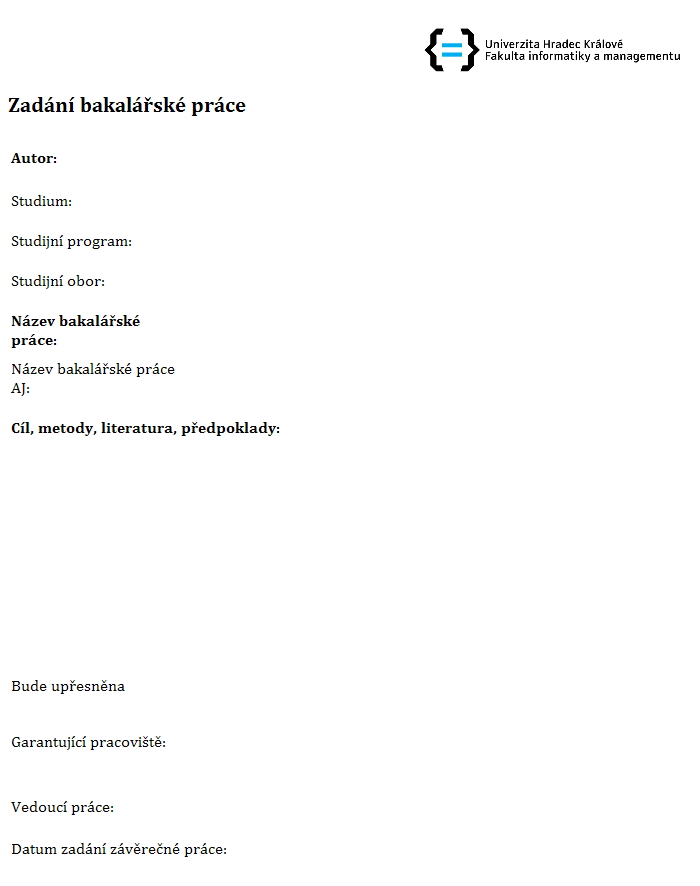
\includepdf[pages=-, offset=20 -50, width=20cm]{images/assignment.png}

\end{document}
